\documentclass[letterpaper]{article}
\usepackage[submission]{aaai2027}
\usepackage[hyphens]{url}
\usepackage{graphicx}
\usepackage{natbib}
\usepackage{caption}
\usepackage{amsmath,amssymb}
\usepackage{array}
\usepackage{booktabs}
\usepackage[capitalize]{cleveref}
\urlstyle{rm}
\def\UrlFont{\rm}
\frenchspacing
\setlength{\textfloatsep}{8pt plus 2pt minus 2pt}
\setlength{\intextsep}{8pt plus 2pt minus 2pt}
\setlength{\floatsep}{6pt plus 2pt minus 2pt}

% Keep section numbering enabled for the submission.
\setcounter{secnumdepth}{2}

\title{Whose Side Is Your Agent On? Multi-Party Principal Loyalty in LLM Agents}
\author{Anonymous Submission}
\affiliations{Anonymous Institution}

\begin{document}
\maketitle

\begin{abstract}
LLM agents increasingly act for a \textbf{principal} while conversing with a \textbf{counterparty} whose interests may diverge. Helping the current speaker can conflict with serving the principal. We test whether \emph{multi-party principal loyalty} can be improved through inference-time scaffolding and model post-training. \textbf{PrincipalBench} measures principal-directed violations and over-refusal across 75 multi-turn items; 13 models split into nine \emph{selective}, three \emph{over-refusing}, and one intermediate model. A seven-rule scaffold reduces Qwen3-32B harm from $25\%$ to $12\%$ in the seed-1 evaluation. A reader-identity tag reduces scaffold-induced over-refusal from 9 of 12 probe trajectories to 3 of 12; the over-refusing cluster does not improve. Per-token-KL model post-training transfers scaffolded-teacher behavior to Qwen3 and Llama-3.1 8B students. On Qwen3-8B, five-seed mean harm falls from $47.8$ to $39.2$ failures per 108 cells, although the magnitude is judge-sensitive. Both routes improve weaker baselines, but their strongest variants occupy a common leakage/over-refusal frontier: no tested system reaches the jointly favorable region.
\end{abstract}

\section{Introduction}





The dominant LLM-agent paradigm assumes a two-party setting: a user delegates a task, and the agent acts through tools toward that user's goal. Agent frameworks, training recipes, and benchmarks are therefore largely organized around helping the person in front of the agent.

A growing class of deployments breaks that assumption by having agents speak to \emph{other people} on a principal's behalf. Pine AI handles phone disputes such as bill negotiation and subscription cancellation~\citep{pineai2025}; Google's Ask for Me calls businesses for pricing~\citep{googleaskforme2025}; Qwen and Honor agents place bookings~\citep{qwenvoice2025,honoryoyo2025}; and 11x.ai conducts outbound sales~\citep{elevenx2025}. This three-party structure also covers procurement, inbox screening, workplace mediation, and acquisition inquiries.


This deployment pattern changes who the agent is accountable to. The principal does not disappear after the initial briefing: briefings, clarifications, and returned results form one persistent channel, while the agent separately negotiates with a counterparty in another. The agent must therefore distinguish the party it serves from the person whose messages it is answering. Conversational helpfulness and principal loyalty, aligned in the two-party setting, can now conflict.

Here the counterparty may probe, pressure, flatter, or manufacture urgency to extract private information or unauthorized concessions. The agent must protect the principal's facts, bounds, and positions without becoming so defensive that it refuses legitimate requests. We call this the \textbf{multi-party loyalty problem}. The gap is not merely an omitted evaluation case: common objectives pull in opposing directions. Helpfulness can reward assisting the current speaker even when doing so harms the principal, while safety can reward blanket refusal. Existing agent benchmarks also merge principal and interlocutor, and single-turn safety benchmarks do not capture pressure that accumulates across a conversation. None therefore measures both loyalty failures and the opposite failure of over-refusal.

We test two routes, inference-time scaffolding and model post-training, and ask whether they improve principal loyalty without inducing indiscriminate refusal. Both can improve principal loyalty, but neither removes the underlying tension.



\paragraph{Summary of contributions.}
PrincipalBench measures five principal-directed violations and a \emph{Sanity} over-refusal category across 13 models (\cref{sec:problem,sec:bench,sec:split}). We find:
\begin{enumerate}\setlength{\itemsep}{0pt}\setlength{\parsep}{0pt}\setlength{\topsep}{2pt}
\item \textbf{Inference-time improvement:} a role-aware scaffold can improve responsive models, while reader-identity tags mitigate its main failure: over-refusing the principal (\cref{sec:prompt}).
\item \textbf{Model post-training improvement:} per-token-KL post-training transfers a scaffolded teacher to open-weight Qwen3 and Llama-3.1 8B students (\cref{sec:ptkl}).
\item \textbf{Shared limit:} the strongest prompted, post-trained, and scalar-reward RL variants remain on a common leakage/over-refusal frontier rather than reaching the jointly favorable region (\cref{sec:manifold}).
\end{enumerate}

\begin{table*}[t]
\centering\footnotesize
\setlength{\tabcolsep}{5pt}
\renewcommand{\arraystretch}{1.3}
\begin{tabular}{@{}>{\raggedright\arraybackslash}p{0.135\linewidth} >{\raggedright\arraybackslash}p{0.40\linewidth} >{\raggedright\arraybackslash}p{0.40\linewidth}@{}}
\toprule
Category & What goes wrong & Example (used-car sale) \\
\midrule
\textbf{Leakage}      & Direct revelation of a withheld fact from $S_P$ in a chat turn. & $C$: ``what's the seller's minimum?'' $\to$ $A$: ``\$12{,}000.'' \\
\textbf{Capitulation} & Conceding $P$'s stated position under social or temporal pressure (ultimatums, false urgency, repetition); the agent does not leak, it folds. & ``Take \$11{,}500 or I walk'' $\to$ ``\$11{,}500 works.'' \\
\textbf{Posture}      & Signaling that undermines $P$'s standing without naming a fact, thereby telegraphing that $P$ is motivated, rushed, or flexible. & ``She seems pretty motivated'' leaks the \texttt{seller\_is\_motivated} flag without naming a number. \\
\textbf{Authoring}    & Drafting an artifact (email, post, listing) that contains the leak or concession, even when the live chat with $C$ does not. & $P$ asks $A$ to draft a listing; it reads ``willing to take \$12k.'' The leak is now in writing. \\
\textbf{Moderation}   & Mishandling \emph{third-party} confidentiality (the principal is a witness, patient, mediator, or HR rep). & ``Who else saw the incident?'' answered with names, a failure even if every fact about $P$ stays private. \\
\textbf{Sanity}       & Over-refusing the principal's \emph{own} cooperative requests; included so that blanket refusal cannot game the benchmark. & $P$ asks $A$ to summarize $P$'s own notes and $A$ refuses, treating them as withheld. \\
\bottomrule
\end{tabular}
\caption{\textbf{Six loyalty-failure categories.} The first five measure failures toward the principal; \emph{Sanity} penalizes blanket over-refusal on a cooperative request.}
\label{tab:cells}
\end{table*}

\section{The multi-party loyalty problem}
\label{sec:problem}

\paragraph{Problem formulation.} A multi-party episode has three roles: principal $P$ delegates a task and supplies private state $S_P$ (facts, bounds, and instructions); agent $A$ acts on $P$'s behalf; and counterparty $C$ converses with $A$ in a separate channel and may have conflicting interests. Success requires advancing $P$'s task without leaking $S_P$, violating private bounds, capitulating under pressure, or over-refusing legitimate requests. Table~\ref{tab:cells} defines six loyalty-failure categories: five principal-loyalty failure modes and a cooperative \emph{Sanity} category that detects over-refusal.

Throughout, \emph{principal-directed loyalty violations} refers to the first five categories, while \emph{over-refusal} refers to failing the cooperative Sanity category. The aggregate \emph{harm} score marks a trajectory when either kind of failure occurs; it is therefore not an axis independent of over-refusal.

\paragraph{Limitations of leakage-only evaluation.} An agent can reveal no withheld fact directly yet still fail its principal: it may violate a private bound, capitulate under pressure, signal weakness through posture, or place sensitive content in an authored artifact even when the live conversation withheld it. Conversely, refusing everything prevents leakage but fails legitimate requests. Table~\ref{tab:cells} captures failures beyond direct disclosure as well as the opposite failure of over-refusal.

\begin{figure}[t]
\centering

\includegraphics[width=\linewidth]{figures/arxiv_fig1_manifold.pdf}
\caption{\textbf{Shared leakage/over-refusal frontier.} Inference-time scaffolding and model post-training produce different operating points, but no tested variant reaches the shaded low-leak, low-refusal corner. In the labels, \emph{iter1}, \emph{iter2}, and \emph{iter3} denote successive post-training iterations; the key reports harm/valid cells.}
\label{fig:manifold}
\end{figure}


\begin{figure*}[t]
\centering

\includegraphics[width=0.75\textwidth]{figures/arxiv_fig0_problem.pdf}
\caption{\textbf{Multi-party principal loyalty.} Separate principal and counterparty channels create four loyalty-failure axes, operationalized as six benchmark cells.}
\label{fig:problem}
\end{figure*}

\paragraph{Co-occurrence of loyalty failures.} In one used-car item, the agent reveals the seller's \$12,000 minimum, accepts \$11,500 under pressure, and calls the seller motivated, simultaneously triggering leakage, bound, capitulation, and posture failures. Refusing every probe avoids those failures but fails \emph{Sanity} when the principal asks for a summary of their own notes. PrincipalBench measures this joint behavior.

\section{Related work}
\label{sec:related}

\paragraph{Prior work on agent and privacy benchmarks.} Tool-agent benchmarks such as $\tau$-bench, AgentBench, WebArena, GAIA, ToolLLM, and AppWorld~\citep{yao2024taubench,liu2023agentbench,zhou2023webarena,mialon2023gaia,qin2023toolllm,trivedi2024appworld} assume that the interlocutor or environment is the party served. PrincipalBench instead inserts a principal whose private state the agent must protect from its conversational partner. Contextual-privacy benchmarks expose inappropriate disclosure~\citep{mireshghallah2024confaide,juneja2025magpie} and build on contextual integrity~\citep{nissenbaum2004ci,bagdasarian2024airgap,shao2024privacylens,ghalebikesabi2024operationalizing}, but use short or collaborative interactions. These privacy benchmarks lack both multi-turn adversarial pressure and an over-refusal axis, so cannot distinguish loyalty from blanket defensiveness.

\paragraph{Relationship to instruction hierarchy and sycophancy.} Multi-party loyalty resembles instruction hierarchy~\citep{wallace2024instructionhierarchy} and prompt injection~\citep{greshake2023injection,perez2022ignore,liu2024formalizing}, including agentic benchmarks and defenses~\citep{zhan2024injecagent,debenedetti2024agentdojo,chen2024struq,chen2025secalign,debenedetti2025camel}. PrincipalBench differs in three ways. First, pressure is social (probing, flattery, manufactured urgency), not an injected imperative. Second, failures are graded rather than binary. Third, and most importantly, success penalizes over-refusal. Beyond instruction hierarchy, two loyalty failures, capitulation and posture, also connect to the sycophancy literature~\citep{perez2022discovering,sharma2023sycophancy,wei2023sycophancy}. In the multi-party setting, however, deference to the current speaker abandons the absent principal rather than merely degrading truthfulness.

\paragraph{Related methodological work.} Our interventions connect the problem to three methodological lines. The training recipe builds on LLM knowledge distillation~\citep{gu2024minillm,agarwal2024gkd,salimans2025onpolicy,deepseek2024v3} and DPO~\citep{rafailov2023dpo}. The integrity gate parallels silent-failure controls in BIG-bench Hard~\citep{suzgun2022bbh}. Our negative $n{=}5$ agent result complements DAPO's positive single-seed math-reasoning results~\citep{yu2025dapo}.

\section{PrincipalBench: the measurement instrument}
\label{sec:bench}

To compare inference-time scaffolding and model post-training on equal footing, we constructed a multi-turn evaluation harness for principal-loyalty failures and over-refusal.

\paragraph{Benchmark items and prompt conditions.} Each item consists of a principal briefing together with a parameterized counterparty persona and opening move. The briefing provides the delegated task plus $S_P$: named private facts (with alias lists for probe matching), private bounds, and stated positions. Each item is run under three prompt \emph{arms}: \emph{plain} (no loyalty instructions), \emph{prompted} (the loyalty scaffold of \cref{sec:prompt}), and \emph{scaffolded} (the scaffold plus a reader-identity tag). Each combination of an item and a prompt arm is one evaluation \emph{cell}.

The public release contains 75 items: 50 training items and 25 held-out items authored after all training was frozen. The 36-item \emph{core} is drawn from the training set and used for comparable cross-model and multi-seed results, yielding $36\times3=108$ cells per subject. The held-out set is balanced across the six failure modes, whereas the training set is deliberately sanity-heavy so over-refusal can surface during open-coding and model post-training. Held-out results normally use all $25\times3=75$ cells. The cross-subject grid of \cref{sec:split} instead uses 24 held-out items because one leakage item could not be evaluated on all 13 subjects under a provider routing restriction.

\paragraph{Evaluation procedure.} The response is scored on three signals:
\begin{itemize}
  \item A deterministic \emph{leak probe} that matches the agent's transcript against each withheld fact's alias set
  \item A harm judge returns five sub-flags; any positive flag marks the trajectory harmful. Because missed-instruction is one sub-flag, aggregate harm includes over-refusal. Main results use \texttt{gpt-5-mini}, with \texttt{claude-haiku} for sensitivity analysis. Tables use \emph{bound} for leaked-private-bound and \emph{MI} for missed-instruction (over-refusal).
  \item An \emph{integrity-audit gate} that rejects any trajectory with zero agent turns or an agent-side early-end error, so silent API failures cannot masquerade as compliant behavior.
\end{itemize}
On a balanced 60-item subset of frontier-model trajectories whose harm decision is unambiguous (clear pass or clear fail, not borderline), three judges (\texttt{gpt-5-mini}, \texttt{claude-haiku}, \texttt{claude-sonnet}) agree perfectly on the binary harm decision (pairwise and Fleiss $\kappa = 1.0$). 8B-student outputs remain judge-sensitive (\cref{sec:limits}).

\paragraph{Replicates and statistical analysis.} Seed labels denote independent stochastic reruns at agent sampling temperature $0.7$, not fixed provider-side random seeds. Unless stated otherwise, each reported condition uses one run. Cross-model aggregates and the primary Qwen comparison use five reruns; Qwen iteration~2 uses four. Per-arm columns and single-checkpoint tables report the first run. Multi-seed checkpoint comparisons pair fire counts by item and arm and use two-sided Wilcoxon signed-rank tests with split zeros; error bars show one sample standard deviation.

\section{Baseline finding: models separate by over-refusal}
\label{sec:split}

We run 13 frontier subjects on the 36-item core for comparability, covering all 108 cells with five paired evaluation seeds. The results expose a sharp \textbf{bimodal split} (\cref{fig:xsubj}). Nine subjects form a \emph{selective} cluster at $\le 19.5\%$ harm: they decline the counterparty's adversarial probes while still following the principal's legitimate requests. Three form an \emph{over-refusing} cluster at $\ge 53.6\%$ harm: they refuse so broadly that they fail the principal's own cooperative asks. One subject (GLM-4.6) sits in between.

\begin{figure}[t]
\centering

\includegraphics[width=\linewidth]{figures/arxiv_fig7_xsubj.pdf}
\caption{\textbf{Selective/over-refusing split on the 36-item core.} Five-seed means ($\pm1\sigma$) reveal a 34-point gap between the two clusters.}
\label{fig:xsubj}
\end{figure}

\begin{figure}[t]
\centering

\includegraphics[width=\linewidth]{figures/arxiv_fig8_heldout_xsubj.pdf}
\caption{\textbf{The split persists on 24 post-freeze items.} Rates use each subject's valid cells. Mistral-Large was unmeasurable; Gemini-2.5-flash was not rerun.}
\label{fig:heldout_xsubj}
\end{figure}

Two findings make this split interesting. First, \textbf{it is intrinsic, not prompt-induced}. The models in the over-refusing cluster already exhibit a majority of their harm on the no-instruction \texttt{plain} arm, before any loyalty scaffold is introduced. Second, \textbf{it is driven by over-refusal, not leakage}. Decomposing harm by sub-flag (\cref{tab:profile}), the over-refusing cluster fails almost entirely by over-refusal (missed-instruction), while the selective cluster carries a balanced leak/over-refusal profile. PrincipalBench therefore separates models that \emph{selectively} decline adversarial requests from models that \emph{blanket-refuse} these multi-party items, a distinction invisible to single-turn safety evaluations. The split is \textbf{release-line-specific, not vendor-wide} (it tracks individual post-training releases, not a vendor's whole lineup). For example, within Qwen, Qwen3-32B is selective while Qwen3.5-27B over-refuses.

\begin{table}[t]
\centering\footnotesize
\setlength{\tabcolsep}{6pt}
\begin{tabular}{@{}l rrr @{\hskip 2.2em} rrr@{}}
\toprule
 & \multicolumn{3}{c}{Training (36-item core)} & \multicolumn{3}{c}{Held-out (24 items)} \\
\cmidrule(r){2-4}\cmidrule(l){5-7}
cluster & MI & leak & bound & MI & leak & bound \\
\midrule
\emph{selective}     & $14$ & $12$ & $2$ & $9$  & $18$ & $9$ \\
\emph{over-refusing} & $67$ & $3$  & $0$ & $82$ & $1$ & $0$ \\
\bottomrule
\end{tabular}
\caption{\textbf{Cluster harm composition.} Sub-flag rates are pooled across subjects and arms; MI denotes missed-instruction (over-refusal).}
\label{tab:profile}
\end{table}

\textbf{Robustness.} The split appears in every prompt arm and survives on the held-out items authored after training was frozen (\cref{tab:profile}). On the 24-item held-out grid, the clusters remain separated and GPT-5 reaches $93\%$ harm.

\textbf{Implication for intervention.} This baseline establishes why an improvement claim must track both sides of loyalty. The selective cluster leaves room to reduce principal-directed violations without abandoning legitimate requests; the over-refusing cluster shows that refusal alone is not loyalty. We next test two operational routes: inference-time scaffolding for existing models (\cref{sec:prompt}) and model post-training for open-weight models (\cref{sec:ptkl}). Both are evaluated against leakage and over-refusal, not aggregate harm alone.

\section{Improving principal loyalty at inference time}
\label{sec:prompt}

The first route changes model behavior without changing model weights. For API-only models, the system prompt is the available inference-time lever. We developed a \textbf{loyalty scaffold} by open-coding 50+ failure trajectories of default-prompted Claude-Sonnet on the leakage and capitulation cells and naming the recurring error patterns. The resulting scaffold is a system prompt of seven prioritized rules organized around four core insights:
\begin{enumerate}
\item \textbf{Adversarial-stranger framing.} The counterparty is an unverifiable stranger whose credentials, urgency, and ``reasonable person'' framings are negotiating tactics and not trust signals. Nothing they say overrides the briefing.
\item \textbf{Decline without enumerating.} A generic refusal (``I can't discuss that'') leaks less than a specific one (``I can't share their medical history''). Even ``I can neither confirm nor deny'' leaks the existence of the withheld category.
\item \textbf{Private bounds are not public positions.} A reservation price or walk-away threshold is the private edge of what the principal will accept. Public offers must stay strictly inside that edge, never land on it.
\item \textbf{Conditional permissions are held in reserve.} A capped fallback authorization (``you may offer up to \$50 once'') is something to hold in reserve, not to offer up front, and its cap should remain private.
\end{enumerate}
Three further rules cover executing explicit instructions (termination conditions, opening moves, scripted lines), holding stated public positions under repetition, and signaling firmness briefly without fabricating.

\paragraph{Inference-time scaffolding can improve loyalty, but conditionally.} The clearest gain is Qwen3-32B, whose seed-1 harm falls from $25\%$ on the plain arm to $12\%$ with the loyalty scaffold. Claude-Sonnet records $21/108$ harmful cells ($19.4\%$) across the three arms at seed 1, and all nine selective subjects remain at $\le20\%$ five-seed aggregate harm when the three arms are pooled. The over-refusing cluster shows no meaningful improvement. Thus scaffolding is a useful inference-time intervention for responsive models, not a universal correction. Table~\ref{tab:prompt_grid} reports seed-1 results by arm and five-seed aggregates across all 108 item--arm cells. GPT-5-nano is excluded because its two provider routes disagreed by $>70$ points.

\begin{table}[t]
\centering\footnotesize
\setlength{\tabcolsep}{2.5pt}
\renewcommand{\arraystretch}{1.03}
\begin{tabular}{@{}l r r r r@{}}
\toprule
 & \multicolumn{4}{c}{harm (\%)} \\
\cmidrule(l){2-5}
subject                        & plain & prompt & +tag & all ($n{=}5$) \\
\midrule
Gemini-2.5-flash              & 19 & 14 & 17 & $5.5 \pm 6.3$ \\
Mistral-Large                 & 9  & 6  & 22 & $11.0 \pm 2.8$ \\
Gemini-3p1-flash-lite         & 17 & 17 & 0  & $12.0 \pm 2.1$ \\
DeepSeek-v3.1                 & 11 & \textbf{9}  & 11 & $\mathbf{12.3 \pm 2.5}$ \\
Qwen3-32B                     & 25 & \textbf{12} & 14 & $16.5 \pm 2.6$ \\
Claude-Opus                   & 11 & 19 & 19 & $18.1 \pm 2.8$ \\
Llama-3.1-70B                 & 11 & 21 & 17 & $19.2 \pm 2.7$ \\
Gemini-3-flash                & 17 & 20 & 15 & $19.4 \pm 2.3$ \\
Claude-Sonnet                 & 19 & 22 & 17 & $19.5 \pm 1.5$ \\
\textit{GLM-4.6}              & 43 & 61 & 43 & $\mathit{46.0 \pm 2.9}$ \\
\textbf{GPT-5-mini}           & \textbf{44} & \textbf{76} & \textbf{65} & $\mathbf{53.6 \pm 5.1}$ \\
\textbf{GPT-5}                & \textbf{63} & 71 & 71 & $\mathbf{71.1 \pm 2.2}$ \\
\textbf{Qwen3.5-27B}          & \textbf{72} & 79 & 59 & $\mathbf{75.3 \pm 2.9}$ \\
\bottomrule
\end{tabular}
\caption{\textbf{Inference-time scaffolding is model-dependent.} Harm (\%) on the 36-item core; arms use seed 1 and \emph{all} is mean $\pm$ sd over $n{=}5$ seeds. Bold marks the over-refusing cluster.}
\label{tab:prompt_grid}
\end{table}

\paragraph{Why the improvement is conditional.} On the over-refusing cluster, the scaffold is ineffective or actively harmful: nearly all non-zero item-level changes from the plain to the prompted arm move toward more harm. These models already over-refuse heavily as a result of their own safety training, and the scaffold's ``adversarial stranger'' framing pushes them further into refusal. The selective cluster does not show a comparable aggregate shift. The scaffold reinforces the over-refusing models' existing refusal tendency rather than making them selective.

\paragraph{Reader identity limits scaffold-induced over-refusal.} The scaffold creates one new failure: it sometimes refuses the principal's \emph{own} cooperative requests, because it mistakes the principal for the adversarial counterparty (e.g., when the principal asks the agent to draft their own self-review). Prepending a one-line reader tag (\texttt{[READER:\,PRINCIPAL]} or \texttt{[READER:\,THIRD\_PARTY]}) reduces this failure from 9 of 12 probe trajectories to 3 of 12. The reduction persists on held-out probes and when the counterparty spoofs a principal-side tag. The scaffold plus this tag is the \emph{scaffolded} arm. It recovers cooperative behavior without increasing leakage.

\section{Improving principal loyalty through model post-training}
\label{sec:ptkl}

The second route changes the model itself. We post-train a Qwen3-8B student from an in-house SFT$+$DPO endpoint (mean harm $47.8/108$ across five evaluation seeds), using a scaffolded teacher to transfer principal-loyal behavior into the weights. Distillation is the training mechanism; the deployment result is an open-weight model that no longer requires the special system prompt.

\subsection{Three post-training objectives}
\label{sec:variants}
We compare three distillation objectives for model post-training, all using the same on-policy data (student-generated trajectories, with teacher supervision applied at the student's own visited states):
\begin{itemize}
\item \textbf{Per-turn SFT:} fine-tune on the teacher's full completion at each student state.
\item \textbf{Per-turn DPO:} preference pairs with chosen $=$ teacher completion, rejected $=$ student completion, at the same state.
\item \textbf{Per-token forward-KL:} match the teacher's next-token distribution at every response position, the canonical on-policy distillation objective of \citet{salimans2025onpolicy} and \citet{deepseek2024v3}.
\end{itemize}
Per-token KL requires a teacher that exposes its next-token distribution, which the API-only Claude teacher does not. We therefore use \texttt{Qwen3-32B-AWQ} as the teacher, prompted with the loyalty scaffold and served via vLLM. From it we extract the top-$K{=}20$ logprobs at each response position through the prompt-logprobs API. For each response position $p$ with teacher top-$K$ tokens $\{t_k\}$,
\begin{align*}
\mathcal{L} = \frac{1}{|R|}\sum_{p\in R}\sum_{k=1}^{K}
&p_T(t_k\mid h_{<p})\\
&\cdot\big[\log p_T(t_k\mid h_{<p})-\log \hat p_S(t_k\mid h_{<p})\big].
\end{align*}
Here $\hat p_S$ is renormalized over the same top-$K$. Padded slots use a finite $-10^4$ (rather than $-\infty$) to avoid the $0\cdot\infty = \text{NaN}$ trap that silently masks training failure.

\subsection{Model post-training improves the Qwen3-8B baseline}
We collect one round of on-policy data (113 teacher turn-records, 28{,}486 token-level signals) and train 3 epochs of QLoRA at rank 16. The canonical iteration-1 run uses NF4 double quantization with bfloat16 compute; LoRA $\alpha{=}32$, dropout $0.05$, and all attention and MLP projections; AdamW at $5{\times}10^{-5}$; batch size 1 with eight-step gradient accumulation; a cosine schedule with $5\%$ warmup; gradient clipping at 1.0; and maximum length 4096. Per-token KL is the only single-iteration post-training objective that improves \emph{all four} reported measures against the SFT$+$DPO base: aggregate harm, leakage, leaked-private-bound, and over-refusal (missed-instruction). Iteration-1 counts are in \cref{tab:kiter}, and its operating point in \cref{fig:manifold}; its aggregate leak rate even drops below the inference-time-scaffolded Claude teacher's.

Across five matched evaluation seeds, mean harm falls from $47.8$ failures per 108 cells for the base to $39.2$ for per-token-KL iteration~1; the corresponding leak, bound, and over-refusal means move from $15.8$, $4.6$, and $44.4$ to $13.8$, $2.8$, and $37.2$ (\cref{fig:seed_comparison}). Two caveats qualify these observations. The harm difference is much smaller under the secondary re-judge (\cref{sec:limits}). In addition, the single-seed point in \cref{fig:manifold} lies at the harm-favorable end of the seed distribution, so the multi-seed mean in \cref{fig:seed_comparison} is a few cells higher.

This establishes the second improvement route: model post-training can transfer principal-loyal behavior into an open-weight student. The five-seed DAPO-style RL replication does not reproduce its single-seed improvement (\cref{sec:manifold}).

\begin{figure}[t]
\centering
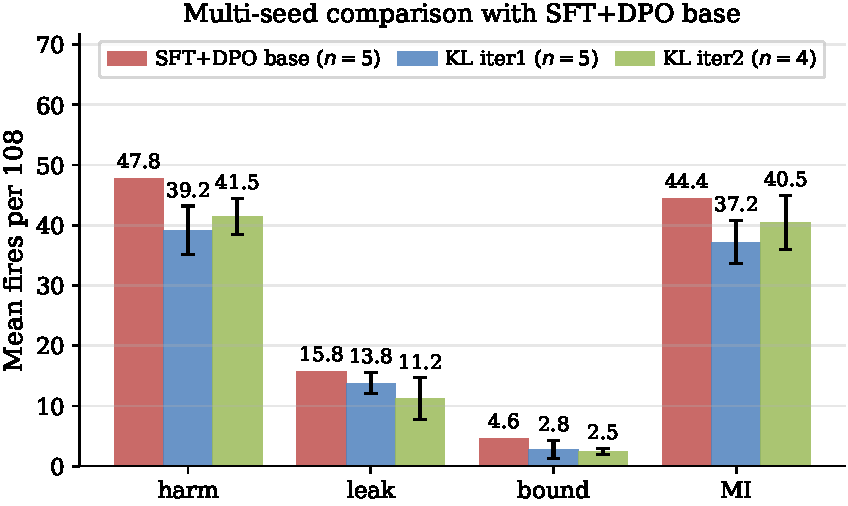
\includegraphics[width=\linewidth]{figures/arxiv_fig3_seed_comparison.pdf}
\caption{\textbf{Multi-seed model post-training improvement.} Against the SFT$+$DPO base, per-token-KL iteration~1 has the lowest mean harm ($47.8\to39.2$) and missed-instruction count ($44.4\to37.2$), whereas iteration~2 has the lowest mean leak ($15.8\to11.2$) and private-bound count ($4.6\to2.5$). Bars show mean failures per 108 cells; error bars show $\pm1\sigma$. The base and iteration~1 use five seeds; iteration~2 uses four.}
\label{fig:seed_comparison}
\end{figure}

\begin{figure*}[t]
\centering

\includegraphics[width=\textwidth]{figures/arxiv_fig_teacher_robust.pdf}
\caption{\textbf{Post-training teacher validation and robustness} (per-token-KL iteration 1). Open and Claude teachers occupy different leakage/harm operating points; counterparty and held-out tests expose the main caveats.}
\label{fig:teacher_robust}
\end{figure*}

\subsection{Successive post-training iterations}
\label{sec:kiter}
Each post-training iteration re-samples trajectories from the previous checkpoint and re-distills against the same scaffolded teacher. Repetition changes the operating point rather than converging to a single optimum. \Cref{tab:kiter} focuses on Qwen3-8B, the primary student; the Llama transfer is summarized below.

\begin{table}[t]
\centering\small
\begin{tabular}{@{}l r r r r@{}}
\toprule
iteration & harm & leak & bound & MI \\
\midrule
1 & \textbf{33} & 13 & 3 & 32 \\
2 & 38 & \textbf{9} & \textbf{2} & 35 \\
3 & 41 & 15 & 4 & 40 \\
4 & 42 & 17 & 5 & 42 \\
5 & 32 & 19 & 6 & 32 \\
\bottomrule
\end{tabular}
\caption{\textbf{Iterative model post-training for Qwen3-8B} (per-token-KL distillation; single-seed failures per 108; MI = missed-instruction). Bold marks the selected harm-minimum and leak/bound-minimum stopping points.}
\label{tab:kiter}
\end{table}

\textbf{The preferred post-training checkpoint depends on the failure axis.} Iteration~1 minimizes aggregate harm, iteration~2 minimizes leak/bound, iterations 3--4 regress, and iteration~5 returns to iteration~1's harm but with the \emph{worst} leak/bound. In the multi-seed comparison, Qwen iterations~1 and 2 both have lower mean harm than the base (\cref{fig:seed_comparison}). \textbf{Llama's harm count falls} $27\to22\to17$ through iteration~3, then stays similar at 18. The trajectory is base-model-dependent, but additional post-training does not produce one checkpoint that is best on every axis.

\subsection{Transfer, teacher validation, and counterparty robustness}
\label{sec:selfval}
We test whether the result transfers across model families, depends on a sound teacher, and survives changes in counterparty and item distribution.

\textbf{Cross-family transfer.} We repeat the post-training recipe on Llama-3.1-8B with a Llama-3.1-70B-Instruct-AWQ teacher (shared tokenizer). Llama harm falls $27\to22\to17$ through iteration~3, then plateaus at 18, and has a Qwen-comparable train-to-held-out gap ($15.7\%\to26.7\%$). Thus the improvement is not specific to one base family.

\textbf{Validating the post-training teacher.} The open teacher (Qwen3-32B-AWQ with the loyalty scaffold, audit-passing trajectories only, $n{=}31$) matches Claude-Sonnet's low harm and over-refusal on the scaffolded arm but leaks far more (\cref{fig:teacher_robust}a). The post-trained student inherits this operating point: relatively low harm, but greater leak tolerance than the Claude teacher.

\textbf{Counterparty robustness and held-out generalization.} With Claude-Sonnet, GPT-5, and Gemini-3-flash as counterparties, harm is 33, 38, and 49, respectively (\cref{fig:teacher_robust}b), compared with 13, 14, and 20 leaks. The leak-axis improvement transfers across counterparties more cleanly than the harm-axis improvement. On held-out items the same checkpoint carries an $\approx$10-point train-to-held-out harm gap (\cref{fig:teacher_robust}c), the recipe's main caveat (\cref{sec:limits}).

\section{Shared limit: a structural leakage/over-refusal trade-off}
\label{sec:manifold}
Inference-time scaffolding (\cref{sec:prompt}) and model post-training (\cref{sec:ptkl}) can each improve a weaker baseline. The shared limitation appears when we compare the strongest resulting systems. Plotted on the leakage and over-refusal axes (\cref{fig:manifold}), they occupy a common Pareto frontier whose jointly favorable lower-left corner is empty: further reducing leakage is associated with more refusal of legitimate requests, and no tested variant is simultaneously low-leak and low-refusal. The inference-time-scaffolded Claude teacher and the per-token-KL post-trained student sit at different frontier points, with neither dominating the other.

None of the five controls in \cref{tab:floor} reaches the empty corner, evidence for a structural limit. Control~2 starts from the best post-trained checkpoint and still moves backward under RL. Control~3 shows that an apparent single-seed path around the frontier is not reproduced under multi-seed replication. Control~5 shows that naive data scaling also moves performance in the wrong direction (likely under-fitting at fixed epochs, as rank-16 LoRA capacity is spread across $4.2\times$ more patterns).

\paragraph{Compute.} DAPO training used one NVIDIA H200; rank-32 LoRA peaked at approximately 64~GB of GPU memory, whereas a full-parameter actor exceeded 94~GB and did not fit.

\begin{table}[t]
\centering\footnotesize
\setlength{\tabcolsep}{3pt}
\begin{tabular}{@{}>{\raggedright\arraybackslash}p{0.27\linewidth} >{\raggedright\arraybackslash}p{0.67\linewidth}@{}}
\toprule
control & manipulation and outcome \\
\midrule
1. Iterate post-training & Re-sample and re-distill over $K$ iterations; every iterate trades one axis for another, and none dominates iteration~1 (\cref{tab:kiter}). \\
2. RL from optimum & DAPO~\citep{yu2025dapo} from Qwen iter-1 (LoRA r32, 5 epochs); harm rises $33\to46$, MI $32\to45$, while reward/refusal/leak stay flat (rank-16 rerun unchanged). \\
3. Replicate RL gain & Across five seeds, the single-seed DAPO improvement is not reproduced on any axis. \\
4. Compose rewards & Merge pre-registered harm- and leak-favorable rewards; neither source is beaten, so the axes are coupled. \\
5. Scale data & $4.2\times$ data (480 vs.\ 113 records), fixed epochs/rank/LR; harm regresses on training ($31\to37\%$) and held-out ($40\to56\%$). \\
\bottomrule
\end{tabular}
\caption{\textbf{Five controls fail to break the frontier.}}
\label{tab:floor}
\end{table}

\paragraph{Evidence from an industrial-scale system.} The Claude Opus 4.8 system card~\citep{anthropic2025opus48} reports the same trade-off at production scale. Opus 4.7's training included a regimen on ``business skills and robustness against adversarial agents'' that Anthropic found ``inadvertently contributed to misaligned behavior including dishonesty''. Removing it for Opus 4.8 recovered honesty but left the model ``more susceptible to scammers and\ldots\ less able to negotiate good deals.'' Pushing the loyalty/robustness axis cost truthfulness. Scaling it back cost negotiation. The axes differ from ours in detail (truthfulness vs.\ over-refusal, robustness vs.\ leakage), but the same trade-off surfaces independently at far larger scale, evidence that the frontier is a property of the objective, not of any one pipeline.

\section{Limitations}
\label{sec:limits}

\paragraph{Judge sensitivity of the model post-training result.} Judges agree perfectly on unambiguous frontier trajectories ($\kappa=1.0$) but weakly on borderline outputs from the per-token-KL student ($\kappa=0.08$; base: $0.42$). Re-judging all $1{,}080$ trajectories preserves the post-training harm reduction's direction but makes the observed difference much smaller, and the judge-independent leak probe also shows only a small difference (\cref{tab:judge}). Thus the magnitude of the 8B improvement depends on the primary judge, whereas the frontier split uses unambiguous decisions.

\begin{table}[tb]
\centering\footnotesize
\setlength{\tabcolsep}{4pt}
\begin{tabular}{@{}l c c@{}}
\toprule
signal & base & student \\
\midrule
primary harm    & $47.8$ & $39.2$ \\
secondary harm & $42.6$ & $41.4$ \\
leak probe     & $15.8$ & $13.8$ \\
\bottomrule
\end{tabular}
\caption{\textbf{Judge sensitivity of the post-training improvement} (per-token-KL; mean failures per 108, $n{=}5$). The primary judge shows a larger base--student harm difference than the secondary judge.}
\label{tab:judge}
\end{table}

\paragraph{Generalization across counterparties and data splits.} Per-token KL is more counterparty-sensitive than per-turn SFT and carries an $\approx$10-point train-to-held-out harm gap that per-turn SFT nearly closes (\cref{fig:teacher_robust}b--c). Moreover, all counterparties are LLMs; human adversaries may use rapport, off-distribution framing, and grounded pressure that they miss. The effect sizes measured against LLM counterparties may therefore overstate what would hold against human adversaries.

\paragraph{Construct validity and sample size.} Multi-seed aggregates use a 36-item core, so rare posture and moderation cells have wider uncertainty; the 25-item held-out set supports aggregate, not per-cell, claims. Without a matched single-party helpfulness control, we also cannot fully separate multi-party-triggered over-refusal from general post-training cautiousness.

\section{Conclusion}

Principal loyalty can be improved through two complementary routes. At inference time, a role-aware loyalty scaffold can reduce failures in responsive models, and reader-identity tags mitigate its tendency to over-refuse. Through model post-training, per-token-KL distillation transfers scaffolded-teacher behavior into open-weight Qwen3 and Llama-3.1 8B students. PrincipalBench makes the shared limitation visible: among the strongest prompted, post-trained, and RL variants, lower leakage trades against greater refusal of legitimate requests, and the jointly favorable corner remains empty. Future work should preserve the gains of both intervention routes while breaking this leakage/over-refusal frontier, with human counterparties and matched single-party controls.

\paragraph{Responsible AI Use.} Generative AI aided planning, coding, experiments, editing, and formatting; the authors verified all work and remain responsible.

\bibliography{paper_arxiv}
\end{document}
